\documentclass{article}
\usepackage[T1]{fontenc}
\usepackage{lmodern}
\usepackage{graphicx}
\usepackage{amsmath,amssymb}
\usepackage[a4paper,margin=2cm]{geometry}
\usepackage[absolute,overlay]{textpos}
\setlength{\TPHorizModule}{1mm}
\setlength{\TPVertModule}{1mm}
\usepackage[indonesian]{babel}
\usepackage{hyperref}
\setlength{\emergencystretch}{2em}
% unit: Halaman 116

\begin{document}

% === Halaman 116 (llm) ===

% (tidak ada teks dari model)

% deskripsi: Screenshot simulator mesin Enigma M3 yang menunjukkan keyboard, roda rotor, dan lampu indikator huruf.
% bbox normalisasi: [0.2110, 0.1570, 0.7580, 0.9530]
\begin{textblock*}{114.87mm}(44.31mm,46.63mm)
\noindent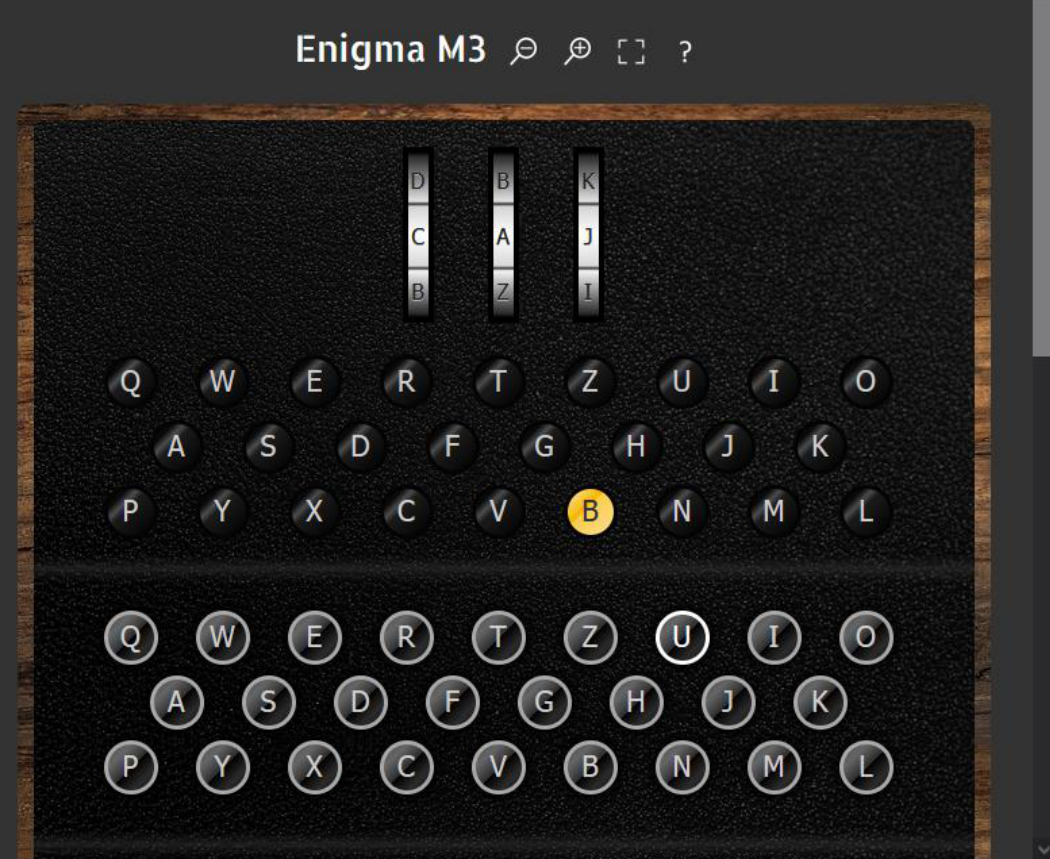
\includegraphics[width=114.87mm,height=236.41mm]{../../images/llm/page_116_img_01.png}%
\end{textblock*}

\end{document}
